%! Author = Philipp Emmenegger
%! Date = 14/07/2021

\section{Programming in Haskell}
\subsection{Functors}
\textbf{The Idea}
\begin{itemize}
    \item Both \textit{Lists} and \textit{Maybe} wrap values of vertain types
    \item We need a generic way to apply functionsto the wrapped values
\end{itemize}

\subsubsection{Definition}
\textbf{Functors} are types that wrap values of other types and allow us to map functions over the wrapped value.
\begin{lstlisting}
class Functor f where
    fmap :: (a -> b) -> f a -> f b
\end{lstlisting}
\textbf{Restriction:} Functors can only map unary functions over them.

\subsubsection{Type Class Laws:}
\begin{itemize}
    \item Concerning the compiler: the only requirement to be a Functor is an implementation of \textbf{fmap} with the proper type
    \item Nevertheless, The \textbf{fmap} function should not change the structure of the Functor, only its elements
    \item Such requirements are expressed as \textit{type class laws}
    \item The compiler will not notice if you violate a type class law, but users of your interface will
\end{itemize}
\textbf{1. fmap has to preserve identity:}
\begin{lstlisting}
fmap id = id
\end{lstlisting}
\textbf{2. fmap has to preserve function composition:}
\begin{lstlisting}
fmap (g . h) = fmap g . fmap h
\end{lstlisting}

\subsubsection{Instances}
\textbf{List} and \textbf{Maybe} are instances of Functor:
\begin{lstlisting}
instance Functor [] where 
    fmap = map

instance Functor Maybe where   
    fmap _ Nothing = Nothing 
    fmap f (Just x) = Just (f x)
\end{lstlisting}
Other instances of \textbf{Functor} in the standard Prelude:
\begin{itemize}
    \item $[]$
    \item Maybe
    \item IO
    \item Option
    \item ((-\textgreater) r)
\end{itemize}

\subsubsection{Usage}
Generalizing \textbf{inc} and \textbf{sqr}:
\begin{lstlisting}
inc :: Functor f => f Int -> f Int 
inc = fmap (+1)

sqr :: Functor f => f Int -> f Int 
sqr = fmap (^2)

-- Usage --
> inc [1,2,3]
[2,3,4]
> inc (Just 1)
Just 2
> inc Nothing
Nothing
\end{lstlisting}

\subsection{Applicative Functors}
\subsubsection{Idea}
\textbf{Provide a generic function to wrap values:}
\begin{lstlisting}
pure :: a -> f a
\end{lstlisting}
\textbf{Provide generalized function application:}
\begin{lstlisting}
(<*>) :: f (a -> b) -> f a -> f b
\end{lstlisting}

\subsubsection{Definition}
\begin{lstlisting}
class Functor f => Applicative f where 
    pure :: a -> f a
    (<*>) :: f (a -> b) -> f a -> f b
\end{lstlisting}

\subsubsection{Instances}
\begin{lstlisting}
instance Applicative Maybe where 
    pure x = Just x
    Nothing <*> _ = Nothing
    (Just f) <*> mx = fmap f mx

instance Applicative [] where 
    pure x = [x]
    fs <*> xs = [f x | f <- fs, x <- xs]
\end{lstlisting}

\subsubsection{Usage}
\begin{lstlisting}
> pure (+) <*> (Just 11) <*> (Just 31)
(Just 42)
> pure (*) <*> [1,2] <*> [3,4]
[3,4,6,8]
> pure (+) <*> [1,2] <*> [3,4]
[4,5,5,6]
> [(*), (+)] <*> [1,2] <*> [3,4]
[3,4,6,8,4,5,5,6]
\end{lstlisting}

\subsubsection{Evaluation}
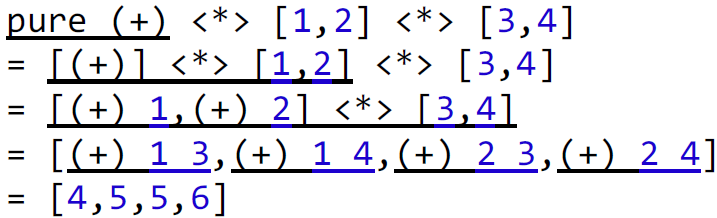
\includegraphics[width=0.6\linewidth]{img/applicative_functors_eval.png}

\subsubsection{Types}
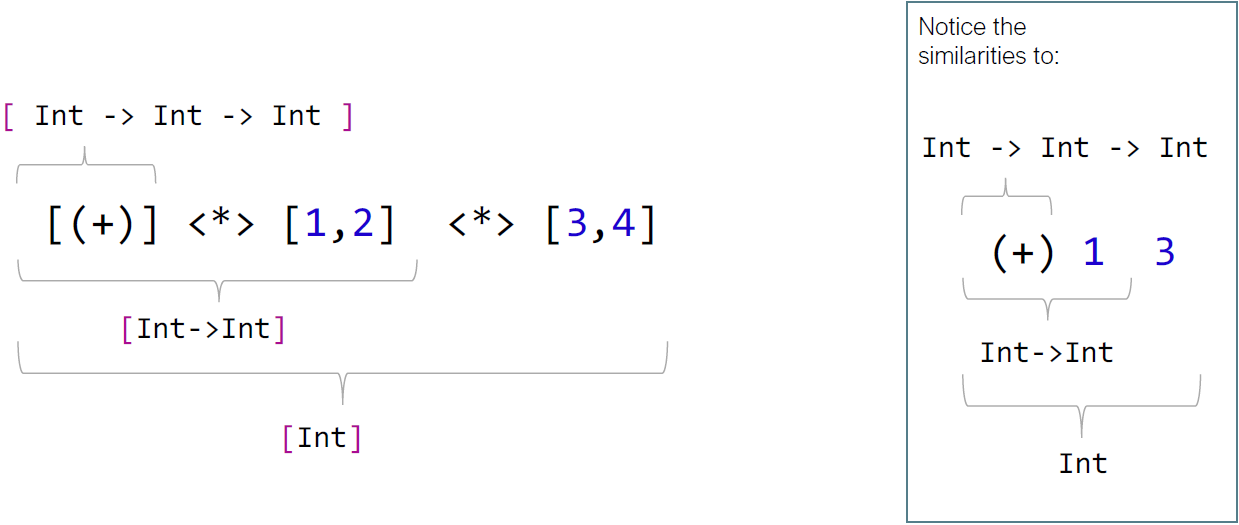
\includegraphics[width=\linewidth]{img/applicative_functors_types.png}

\subsubsection{Type Class Laws}
\textbf{1. Identity: pure has to preserve identity:}
\begin{lstlisting}
pure id <*> x = x
\end{lstlisting}
\textbf{2. Homomorphism: pure has to preserve function application:}
\begin{lstlisting}
pure (g x) = pure g <*> pure x
\end{lstlisting} 
\textbf{3. Interchange: Order of evaluation must not matter when applying an effectful function to a pure argument:}
\begin{lstlisting}
x <*> pure y = pure (\f -> f y) <*> x
\end{lstlisting}
\textbf{4. Composition: $<*>$ must be associative}
\begin{lstlisting}
x <*> (y <*> z) = (pure (.) <*> x <*> y) <*> z
\end{lstlisting}

\subsubsection{The IO Applicative Functor}
\begin{lstlisting}
instance Applicative IO where 
    pure = return
    mf <*> mx = do 
        f <- mf 
        x <- mx
        return (f x)
-- allows for simple composition of IO actions --
getChars :: Int -> IO String 
getChars 0 = return []
getChars n = pure (:) <*> getChar <*> getChars (n-1)
\end{lstlisting}

\subsection{Effectful Programming}
\textbf{Effectful} means that arguments and return values are no longer just plain (pure) values, but many also have so-called \textit{effects}:
\begin{itemize}
    \item The possibility of failure: e.g. option type \textbf{Maybe}
    \item Aggregating multiple results: e.g. using the list type \textbf{[]}
    \item Performing IO: e.g. using the action type \textbf{IO}
\end{itemize}

\subsection{Monads}
\subsubsection{Motivation}
\begin{lstlisting}
-- ADT for expressions --
data Expr = Val Int
    | Div Expr Expr

-- problematic eval fn --
eval (Val n) = n
eval (Div l r = eval l `div` eval r)

-- employ Maybe to fail gracefully --
safediv _ 0 = Nothing 
safediv l r = Just (l `div` r)

-- eval using safediv (ugly AF) -- 
eval (Val n) = Just n
eval (Div l r) = case eval l of
    Nothing -> Nothing 
    (Just x) -> case eval r of
        Nothing -> Nothing 
        (Just y) -> safediv x y

-- eval using Maybe Monad --
eval (Val n) = Just n
eval (Div l r) = do
    x <- eval l
    y <- eval r
    safediv x y
\end{lstlisting}

\subsubsection{The Idea}
\begin{itemize}
    \item We cannot use \textbf{fmap} to simplify \textbf{eval} due to mismatching types
    \item We can exploit the repeating pattern we observed
\end{itemize}
\textbf{Provide a function called:} $(>>=)$ (aka. bind)\\
Binds an effectful value into an effectful function:
\begin{lstlisting}
(>>=) :: m a -> (a -> m b) -> m b
\end{lstlisting}

\subsubsection{Definition}
\begin{lstlisting}
class Applicative m => Monad m where
    return :: a -> m a
    (>>=) :: m a -> (a -> m b) -> m b
\end{lstlisting}


\subsubsection{Instances}
\begin{lstlisting}
instance Monad Maybe where
    Nothing >>= _ = Nothing 
    (Just x) >>= f = f x

instance Monad [] where
    xs >>= f = [y | x <- xs, y <- f x]
\end{lstlisting}

\subsubsection{Evaluation}
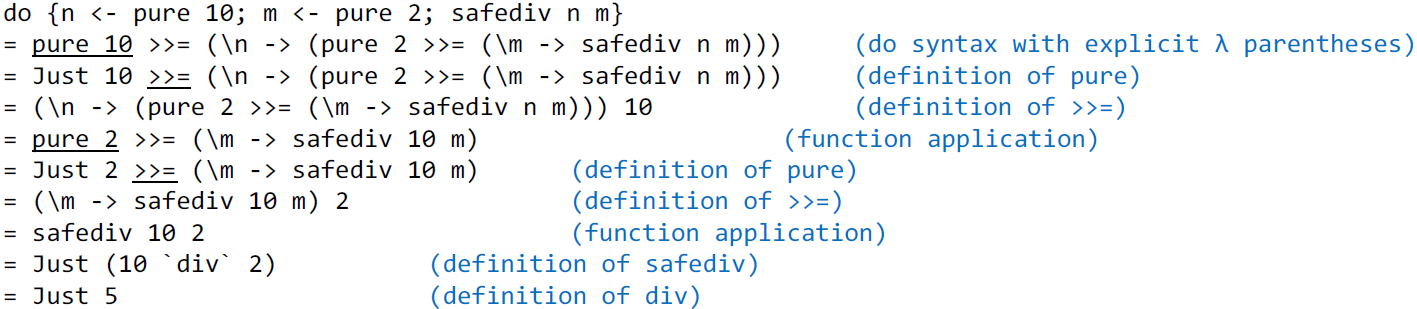
\includegraphics[width=\linewidth]{img/monads_eval.png}

\subsubsection{Types}
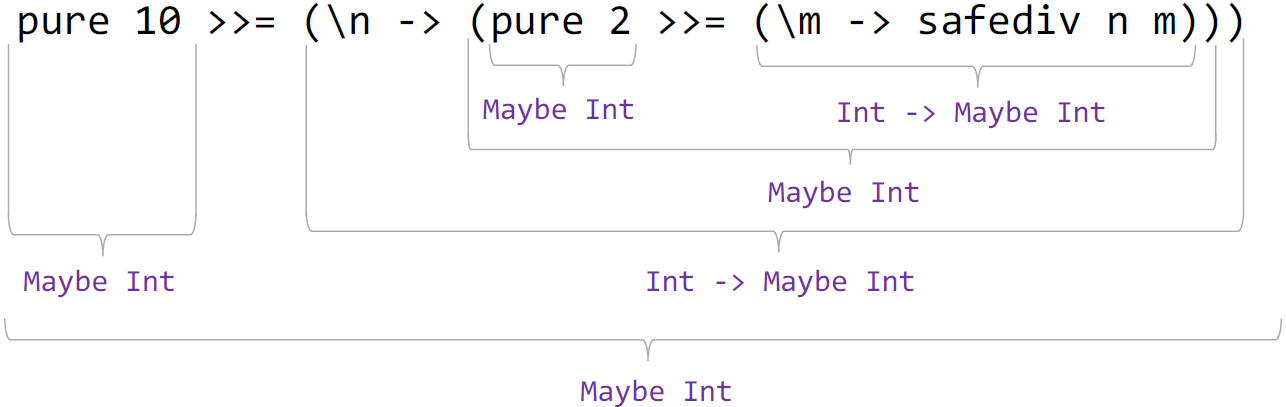
\includegraphics[width=\linewidth]{img/monads_types.png}

\subsubsection{Type Class Laws}
\textbf{1. return is the identity for bind $(>>=)$:}
\begin{lstlisting}
return x >>= f = f x
mx >>= return = mx
\end{lstlisting}
\textbf{2. bind $(>>=)$ must be associative:}
\begin{lstlisting}
(mx >>= f) >>= g = mx >>= (\x -> (f x >>= g))
\end{lstlisting}

\subsection{Overview}
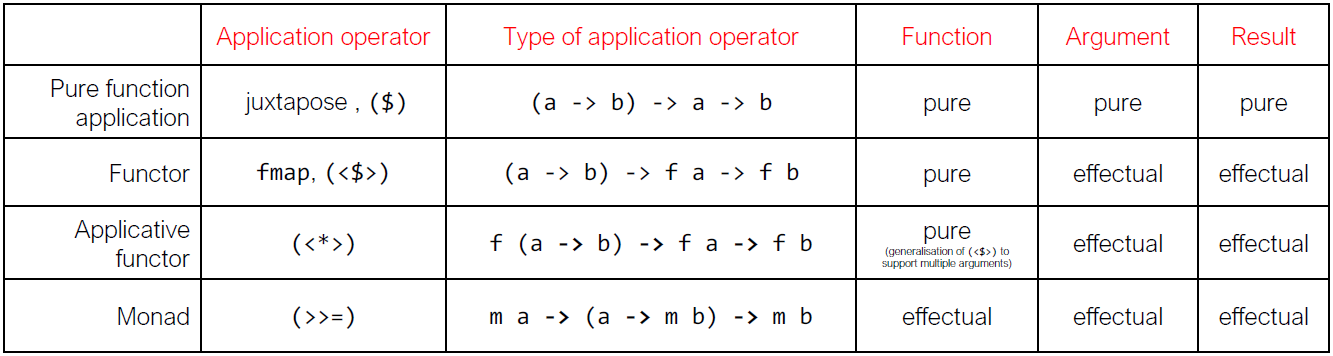
\includegraphics[width=\linewidth]{img/overview.png}